\section{Analyzing the network output}
Find 10 best images for every class => we want to see the best case.

\nblink{nhs-chest-xray/analyze/find\_best\_images.ipynb}
\nblink{nhs-chest-xray/analyze/find\_best\_images\_with\_bounding\_boxes.ipynb}

\nblink{nhs-chest-xray/analyze/accuracy\_per\_class.ipynb}

\section{Applying RISE}
Problem: returned classes from RISE do not match with precalculated classes
=> normalize was not applied on find\_best\_images.
=> use same function on all image loaders

\nblink{nhs-chest-xray/analyze/rise.ipynb}
\nblink{nhs-chest-xray/analyze/rise\_bounding\_boxes.ipynb}

\subsection{Results}
\begin{figure}[h]
\centering
\caption{RISE example 1}
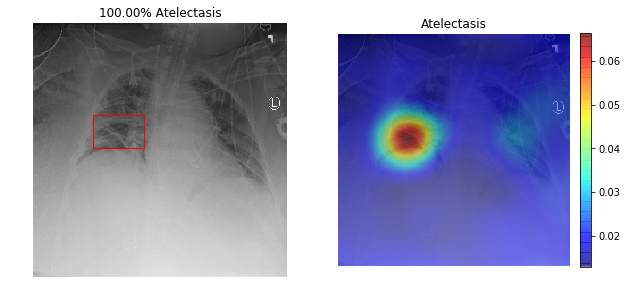
\includegraphics[width=12cm]{chapters/03_classification/images/rise_0.png}
\end{figure}

\begin{figure}[h]
\centering
\caption{RISE example 2}
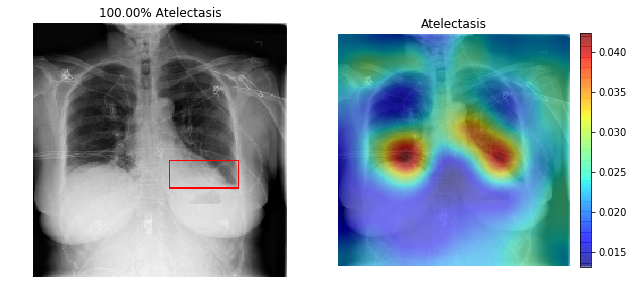
\includegraphics[width=12cm]{chapters/03_classification/images/rise_2.png}
\end{figure}

\begin{figure}[h]
\centering
\caption{RISE example 3}
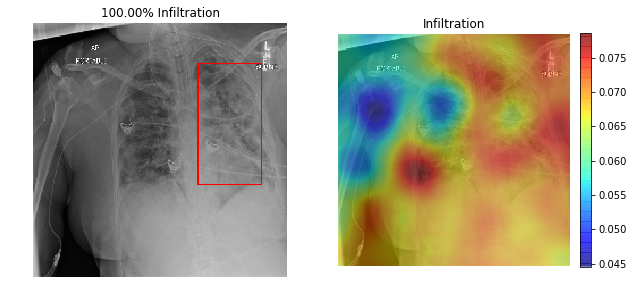
\includegraphics[width=12cm]{chapters/03_classification/images/rise_8.png}
\end{figure}

\subsection{Discussion}
Looks good for most, some (like the last image) are very bad.

\subsection{Conclusion}
Works good for most of the things, returns good quality, returns results for multiple classes at once which is probably helpful for segmentation

\section{Applying LIME}

\nblink{nhs-chest-xray/analyze/lime.ipynb}

\begin{figure}[h]
\centering
\caption{Scan 0 LIME output}
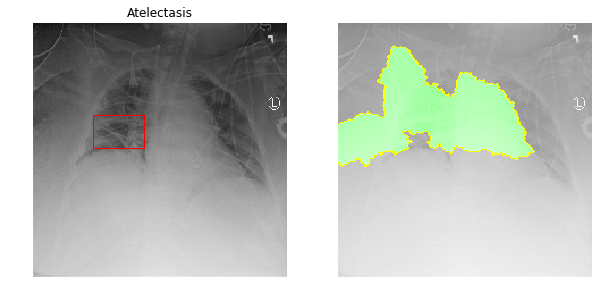
\includegraphics[width=12cm]{chapters/03_classification/images/lime_0.png}
\end{figure}

\begin{figure}[h]
\centering
\caption{Scan 2 LIME output}
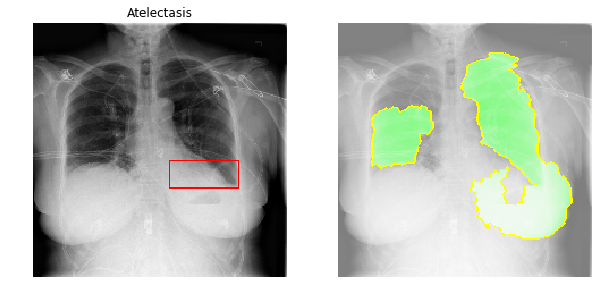
\includegraphics[width=12cm]{chapters/03_classification/images/lime_2.png}
\end{figure}

\begin{figure}[h]
\centering
\caption{Scan 8 LIME output}
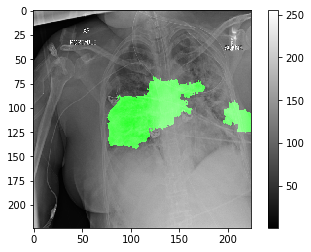
\includegraphics[width=12cm]{chapters/03_classification/images/lime_8.png}
\end{figure}

\subsection{LIME configuration}
\nblink{nhs-chest-xray/analyze/lime\_num\_features.ipynb}

\begin{figure}[h]
\centering
\caption{LIME Superpixel count: 1, 3, 6, 9}
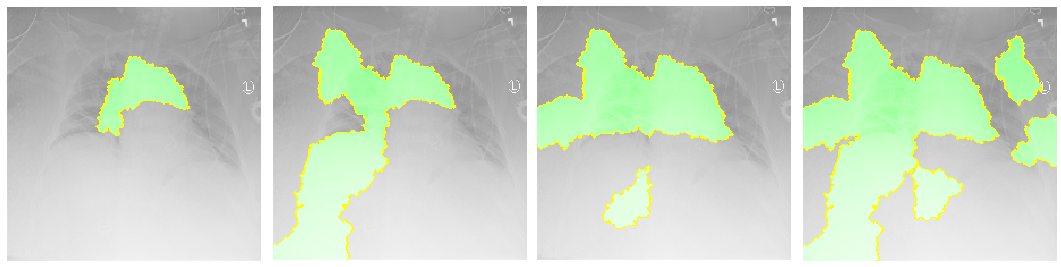
\includegraphics[width=14cm]{chapters/03_classification/images/lime-superpixel.png}
\end{figure}

\section{Applying Grad-CAM}
\nblink{nhs-chest-xray/analyze/grad-cam.ipynb}

